\chapter{Theoretischer Hintergrund}
\label{chap:theoretische_hintergrund}

Um den aktuellen \textbf{Stand der Technik} und die wichtigsten Konzepte im Bereich der Embedded Systems und des 
Machine Learning in der Industrie 4.0 zu untersuchen, wird eine strukturierte \textbf{Literaturrecherche} durchgeführt. 
Diese Methodik gewährleistet eine umfassende und wissenschaftlich fundierte Darstellung des Themas, die auf relevanten 
Fachartikeln \cite{10087221}, Büchern \cite{Soldatos2024} und Konferenzberichten \cite{8119409} basiert. Der Fokus liegt 
auf der Identifizierung und Analyse von Herausforderungen und Lösungsansätzen für die Implementierung von Machine Learning (ML) 
auf Embedded Systems unter den Bedingungen der Industrie 4.0. Durch die strukturierte Recherche werden folgende Kernbereiche 
für das Kapitel ermittelt: die Rolle von Embedded Systems und ML in der Industrie 4.0, spezifische technische Herausforderungen 
sowie Ansätze zur Optimierung von ML-Modellen für ressourcenbeschränkte Umgebungen.


\section{Embedded Systems und Machine Learning in der \Iviernull}

\subsection{Embedded Systems}
\begin{figure}[h]
    \centering
    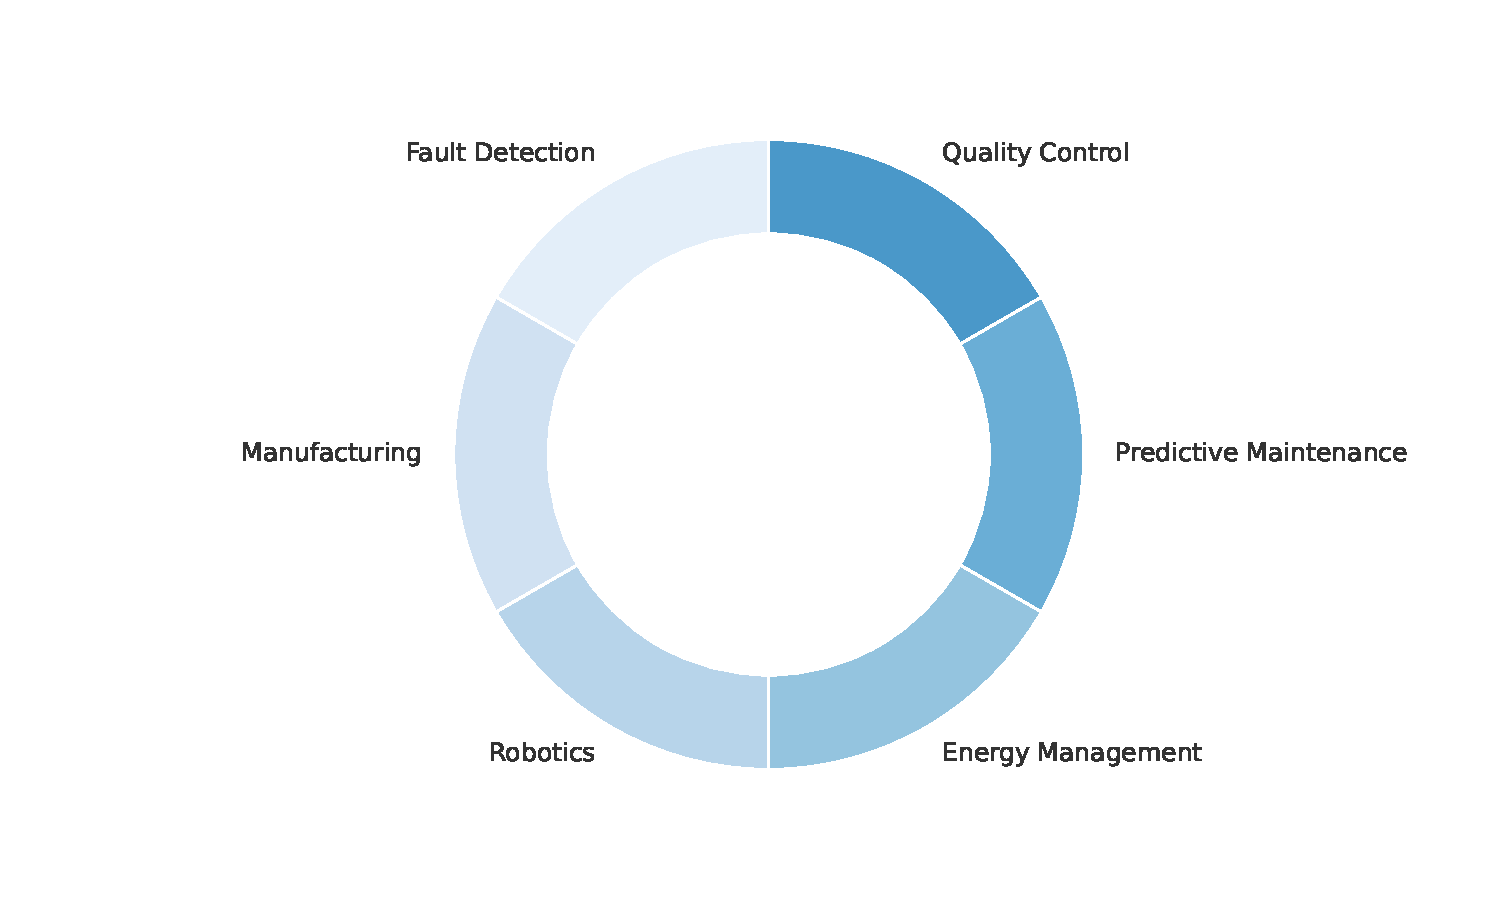
\includegraphics[width=0.5\textwidth]{donut_chart_EmbSys.pdf}
    \caption{Arten von Embedded Systems in der Industrie 4.0} 
    \label{fig:donut_chart_EmbSys}
\end{figure}
Embedded Systems sind spezialisierte Computersysteme, die in größere Maschinen oder Geräte integriert sind,
um spezifische Aufgaben zu erfüllen. Sie sind oft in Umgebungen mit strengen Anforderungen an Zuverlässigkeit, 
Echtzeitfähigkeit und Energieeffizienz im Einsatz. Beispiele für Embedded Systems finden sich in Automobilen, 
medizinischen Geräten, Industrieanlagen und Haushaltsgeräten. In der \Iviernull spielen Embedded Systems eine Schlüsselrolle, 
da sie die intelligente Vernetzung und Steuerung von Maschinen ermöglichen. 

\subsection{\Iviernull}

Der Begriff "Industrie 4.0" beschreibt die vierte industrielle Revolution, die durch die Digitalisierung und Vernetzung 
von Produktionsprozessen gekennzeichnet ist. Diese Transformation ermöglicht die Schaffung \textbf{intelligenter Fabriken}, 
in denen Maschinen und Systeme miteinander kommunizieren und \textbf{autonom} Entscheidungen treffen können. Embedded Systems 
sind dabei das Rückgrat der \Iviernull, da sie die notwendige Hardwarebasis für die Integration von Sensoren, 
Aktoren und Kommunikationsschnittstellen bieten.

\subsection{Machine Learning in der \Iviernull}

\ML ist ein zentraler Bestandteil der \Iviernull, da es die Analyse großer Datenmengen und die Ableitung 
von Entscheidungen in Echtzeit ermöglicht. In Produktionsumgebungen wird \ML zur vorausschauenden Wartung, 
Qualitätskontrolle, Prozessoptimierung \cite{telecom4010011} und vielen weiteren Anwendungen eingesetzt. Dabei müssen ML-Modelle häufig auf 
Embedded Systems ausgeführt werden, um Entscheidungen direkt vor Ort treffen zu können. Dies stellt jedoch besondere Anforderungen 
an die Modellgröße, Rechenleistung und Energieeffizienz.
\begin{figure}[h]
    \centering
    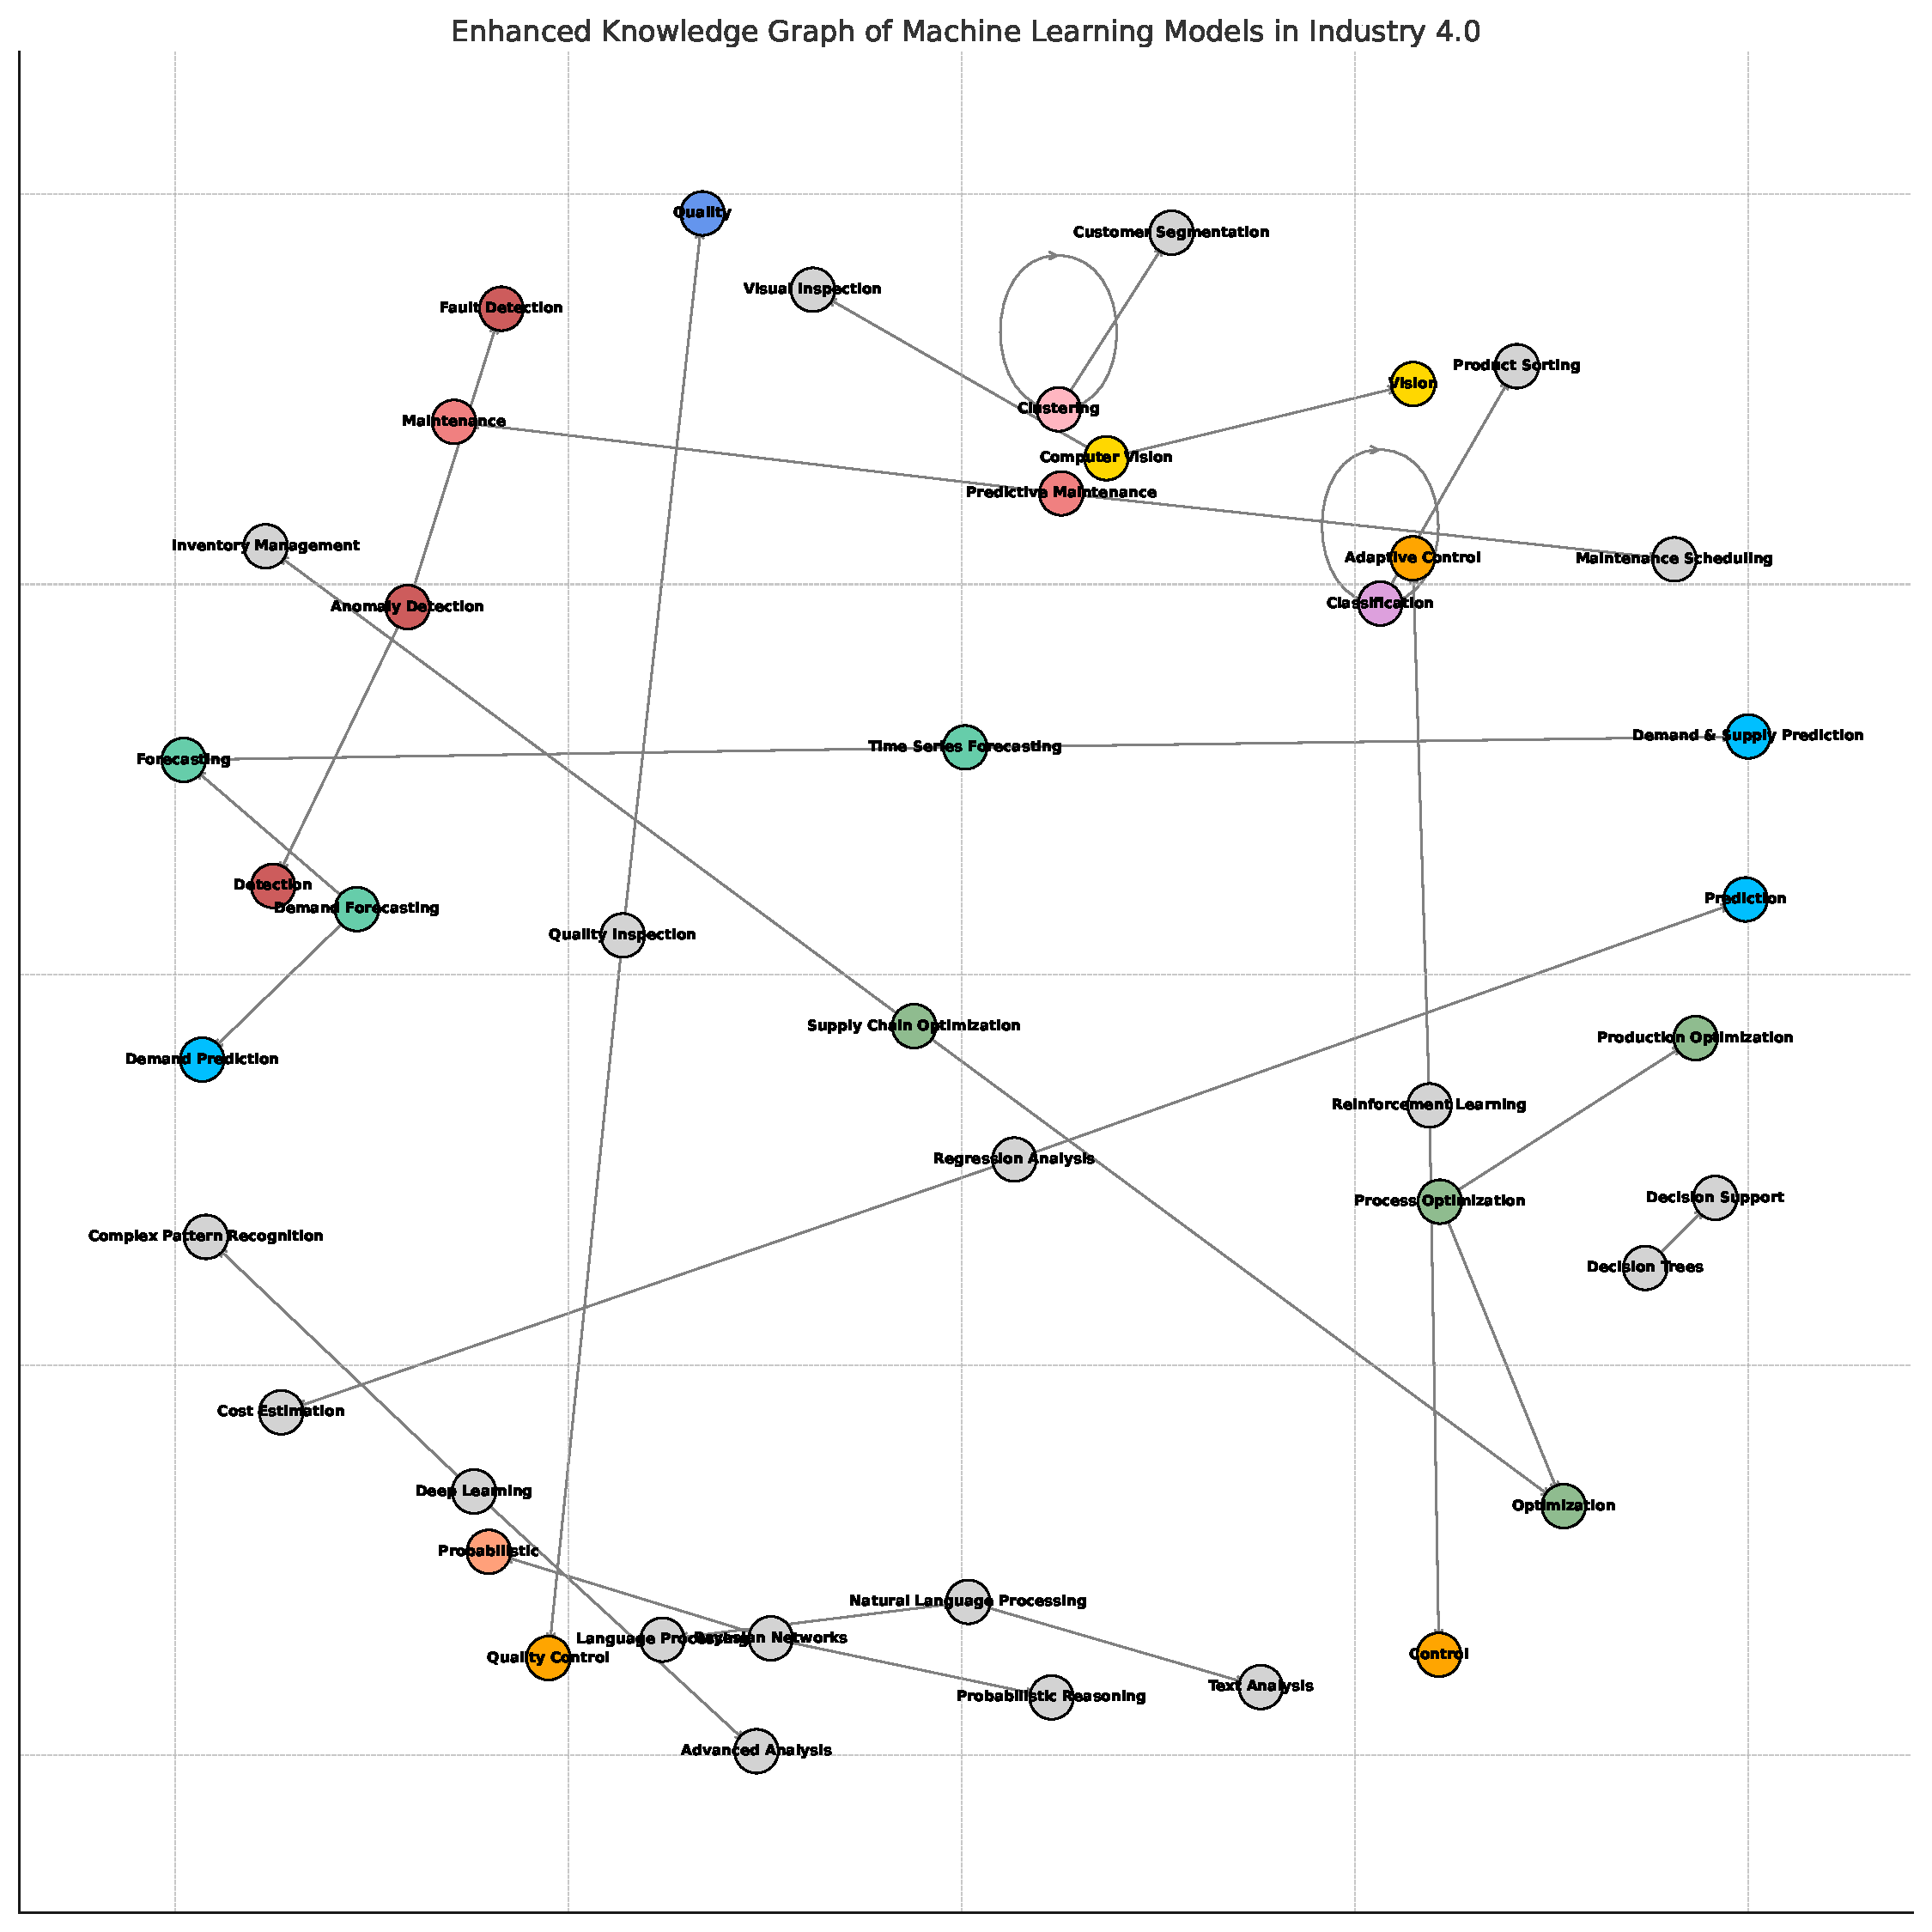
\includegraphics[width=0.7\textwidth]{ml_modelle_KG.pdf}
    \caption{ML Modelle und ihre Anwendungen in der Industrie 4.0}
    \label{fig:ml_modelle_KG}
\end{figure}

\subsection{Herausforderungen bei der Implementierung von \ML auf Embedded Systems}
\subsubsection{Rechenleistung und Ressourcenbeschänkungen}

Ein Hauptproblem bei der Implementierung von \ML auf \Emb ist die begrenzte Rechenleistung und der eingeschränkte Speicherplatz.
Im Gegensatz zu leistungsstarken Servern oder Cloud-Umgebungen verfügen \Emb, inbesondere \SPS und \IPC (IPC), über deutlich weniger 
Ressourcen. \SPS (SPS) sind speziell für industrielle Automatisierungsaufgaben audgelegt und optimiert, haben jedoch nicht die 
Rechenkapazität, um komplexe \ML Algorithmen auszuführen. IPCs sind zwar leistungsfähiger, stoßen jedoch ebenfalls schnell an ihre 
Grenzen, wenn großse ML-modelle oder rechenintensive Aufgaben direkt auf der Hardware ausgeführt werden sollen.
\begin{table}[h!]
    \centering
    \begin{tabular}{|l|l|l|}
    \hline
    \textbf{Aspekt}        & \textbf{SPS (PLC)}                            & \textbf{ML-Computes (AI/ML-Instanzen)}         \\ \hline
    \textbf{Funktion}      & Industrielle Steuerung, Automatisierung       & KI/ML-Modelltraining, Datenverarbeitung        \\ \hline
    \textbf{Beispiele}     & Siemens SIMATIC, B\&R X20                     & AWS P4d, Azure ND H100 v5                      \\ \hline
    \textbf{Leistung}      & Echtzeit, geringe Latenz                      & Hohe Rechenleistung, parallele Verarbeitung    \\ \hline
    \textbf{Hardware}      & ARM/x86-CPUs, I/O-Module                      & NVIDIA-GPUs (A100, H100), TPUs                 \\ \hline
    \textbf{Netzwerk}      & Fieldbus, Ethernet für Steuerung              & InfiniBand, Hochgeschwindigkeits-Ethernet      \\ \hline
    \textbf{Speicher}      & Moderater RAM, Flash                          & Hoher RAM (bis zu 1 TB), SSD/NVMe              \\ \hline
    \textbf{Programmierung} & Ladder-Logik, IEC 61131-3                    & Python, CUDA, ML-Frameworks                    \\ \hline
    \textbf{Skalierbarkeit} & Begrenzt, physische Erweiterung              & Hoch, Cloud-Skalierung über GPUs               \\ \hline
    \textbf{Anwendung}     & Maschinensteuerung, Echtzeitsysteme           & KI, Deep Learning, Big Data                    \\ \hline
    \end{tabular}
    \caption{Vergleich zwischen SPS und ML-Computes}
    \end{table}

\subsubsection{Echtzeitanforderungen}

Viele industrielle Anwendungen erfordern Echtzeitentscheidungen. Das bedeutet, dass die Zeit, die ein ML-Algorithmus für die 
Verarbeitung und Entscheidung benötigt, extrem kurz sein muss. Echtzeitsysteme müssen garantieren, dass eine Etscheidung innerhalb 
einer festgelegtenFrist getroffen wird. Dies stellt eine enorm Herausforderung für ML-Modelle dar, die in der Regel große Datenmengen
verarbeiten und komplexe Berechnungen durchführen. In ressourcebeschränkten Umgebungen wie \Emb kann dies zu significanten Latenzen 
führen, die in Echtzeitsysteme nicht toleriert werden können.

\begin{tcolorbox}[colback=myblue1, colframe=myblue3, coltitle=myblue5, title=Beispiel]
    Ein Produktionsband in einer Automobilfabrik verwendet \ML zur Qualitätsüberwachung von Karosserieteilen. 
    Jedes Teil wird von Kameras gescannt, und die Daten werden in Echtzeit verarbeitet, um Defekte zu erkennen. Wenn das ML-System 
    nicht innerhalb von wenigen Sekunden eine Entscheidung trifft, ob das Teil in Ordnung ist oder aussortiert werden muss, 
    kann das gesamte Produktionsband verzögert werden. Diese Verzögerungen führen zu Produktionsausfällen und erhöhen die Kosten.
    
    \end{tcolorbox}

\subsubsection{Modellkomplexität und Optimierung}

Die Komplexität der ML-Modelle muss für den Einsatz auf \Emb reduziert werden. Moderne ML-Modelle, wie tiefe neuronale 
Netze (Deep Neural Networks, DNNs), sind oft sehr groß und benötigen erhebliche Rechenleistung. Um diese Modelle auf Embedded 
Systemen auszuführen, müssen sie optimiert werden. Techniken wie Model \textbf{Pruning} (das Entfernen von unwichtigen Teilen des Modells) 
und \textbf{Quantisierung} (die Reduktion der Genauigkeit von Modellparametern) \cite{articleQuantization} werden häufig verwendet, um die Modelle kleiner und effizienter 
zu machen. Diese Optimierungstechniken sind jedoch oft mit einem Verlust an Genauigkeit verbunden, was den Einsatz in sicherheitskritischen 
Systemen einschränken kann.

\subsubsection{Energieeffizienz}

In vielen industriellen Anwendungen, insbesondere im Kontext der \Iviernull, spielt die Energieeffizienz eine entscheidende Rolle. 
\Emb sind oft batteriebetrieben oder müssen in energiearmen Umgebungen arbeiten. Das bedeutet, dass ML-Modelle so 
optimiert werden müssen, dass sie möglichst wenig Energie verbrauchen. Der Einsatz energieeffizienter Algorithmen und die Optimierung 
der Hardware, beispielsweise durch die Verwendung von Low-Power-Chips, sind essenziell, um ML-Modelle in eingebetteten Systemen 
langlebig und nachhaltig zu betreiben.

\section{Fazit}

Zusammenfassend lässt sich sagen, dass \Emb und \ML wesentliche Bausteine der \Iviernull sind. 
Die Implementierung von \ML auf \Emb birgt jedoch signifikante Herausforderungen, insbesondere in Bezug auf 
Rechenleistung, Echtzeitanforderungen, Modellkomplexität und Energieeffizienz. Diese Herausforderungen müssen überwunden werden, 
um ML-Modelle effektiv in industriellen Produktionsumgebungen einzusetzen und den Nutzen von intelligenten, autonomen Systemen 
voll auszuschöpfen.